% ============================================================
%  COMPREHENSIVE MANUSCRIPT: FFT-Based Analysis of Phase-Contrast
%  Microscopy Images for Cell Line Characterization and
%  Segmentation Enhancement
% ============================================================
%  Target: Nature Methods / Medical Image Analysis / Bioinformatics
%  Author: Prof. Dr. Md. Enamul Hoque
%  Institution: Shahjalal University of Science and Technology
% ============================================================

\documentclass[11pt,a4paper]{article}

% ---- Packages ----
\usepackage[margin=2.5cm]{geometry}
\usepackage{graphicx}
\usepackage{booktabs}
\usepackage{amsmath,amssymb}
\usepackage{siunitx}
\usepackage{caption}
\usepackage{subcaption}
\usepackage{hyperref}
\usepackage{xcolor}
\usepackage{float}
\usepackage{setspace}
\usepackage{parskip}
\usepackage{multirow}
\usepackage{colortbl}
\usepackage{tikz}
\usepackage{pgfplots}
\usepackage{enumitem}
\usepackage{wrapfig}
\usepackage{makecell}
\usepackage{xspace}
\usepackage{algorithm}
\usepackage{algorithmic}

\usetikzlibrary{shapes,arrows,positioning,calc,decorations.pathreplacing,patterns,fit,backgrounds}
\pgfplotsset{compat=1.18}

\hypersetup{
    colorlinks=true,
    linkcolor=blue!70!black,
    citecolor=blue!70!black,
    urlcolor=blue!70!black
}

\onehalfspacing

% ---- Custom Commands ----
\newcommand{\eg}{e.g.,\xspace}
\newcommand{\ie}{i.e.,\xspace}
\newcommand{\etal}{et~al.\xspace}
\newcommand{\fft}{\textsc{fft}\xspace}
\newcommand{\iou}{\textsc{iou}\xspace}
\newcommand{\svm}{\textsc{svm}\xspace}
\newcommand{\rf}{\textsc{rf}\xspace}
\newcommand{\lr}{\textsc{lr}\xspace}
\newcommand{\pca}{\textsc{pca}\xspace}
\newcommand{\bce}{\textsc{bce}\xspace}
\newcommand{\nii}{\textsc{n2v}\xspace}
\newcommand{\care}{\textsc{care}\xspace}
\newcommand{\debcr}{\textsc{debcr}\xspace}
\newcommand{\piddpm}{\textsc{pi-dddpm}\xspace}
\newcommand{\dog}{\textsc{dog}\xspace}
\newcommand{\lo}{\textsc{lq}\xspace}
\newcommand{\hq}{\textsc{hq}\xspace}

% ---- Title ----
\title{\textbf{Comprehensive Fourier-Domain Analysis and Physics-Informed
Enhancement of Phase-Contrast Microscopy Images:\\
A Multi-Workstream Computational Framework for Cell Line
Characterization, Bandpass Filtering, and Segmentation Enhancement}}

\author{
Prof.~Dr.~Md.~Enamul Hoque\thanks{Corresponding author: \texttt{enamul.physics@sust.edu}} \\
\textit{Department of Physics, Shahjalal University of Science and Technology} \\
Sylhet, Bangladesh
}

\date{\today}

% ============================================================
\begin{document}
\maketitle

% ============================================================
%  ABSTRACT
% ============================================================
\begin{abstract}
We present a comprehensive, multi-workstream computational framework for
Fourier-domain analysis and physics-informed enhancement of phase-contrast
microscopy images. Applied to the LIVECell dataset (3,727 images, 8 cell
lines, 22 time-lapse wells, 258,569 annotated instances), our work
encompasses seven integrated workstreams: (1)~cell density estimation and
spatial spectrum analysis via 2-D fast Fourier transform (\fft) features;
(2)~cell morphology characterization through spectral peak and centroid
analysis; (3)~image quality assessment using isotropy and spectral slope
metrics; (4)~cell line classification from 94-dimensional \fft feature
vectors achieving 81.7\% accuracy (SVM-RBF, 5-fold stratified CV);
(5)~systematic evaluation of 12 bandpass filter types (Ideal, Butterworth,
Gaussian, Chebyshev~I/II, Elliptic, Laplacian-BP, Homomorphic, Gabor,
Difference-of-Gaussians, Trapezoidal, Cosine-tapered) across 8 cell lines
and 4 degradation types (Gaussian noise $\sigma{=}50$, defocus blur
$\sigma{=}4$, illumination shading $\alpha{=}0.5$, combined mild), totaling
over 20,000 segmentation evaluations; (6)~physics-informed deep learning
enhancement models (\debcr, \piddpm, PSF-Learning) integrated with
bandpass filtering, yielding up to 2$\times$ improvement over
filter-only approaches; (7)~U-Net segmentation with 5-fold
cross-validation; (8)~BBBC005 blur-level analysis across 25 degradation
levels; (9)~cross-modality transfer analysis; and (10)~cell-line-adaptive
enhancement with quality-aware model selection. Key findings: (i)~total
\fft power correlates strongly with cell density ($r{=}0.751$, $p{<}0.001$);
(ii)~no single bandpass filter is universally optimal---\dog excels for
segmentation (3/8 cell lines), Homomorphic for illumination correction
(2/8), and Butterworth provides the safest default; (iii)~filter
improvements on low-quality images are 10--100$\times$ smaller than on
high-quality images, motivating physics-informed enhancement as a
preprocessing step; (iv)~adaptive, cell-line-specific filter selection
improves mean \iou by $+$0.130 over fixed filtering; (v)~the
\debcr$+$\dog combination achieves the best overall enhancement-filtering
pipeline. All code, trained models, and results are available at
\url{https://github.com/mjonyh/microscopic_images}.
\end{abstract}

\textbf{Keywords}: Fourier transform, phase-contrast microscopy, cell
segmentation, cell line classification, bandpass filtering, physics-informed
neural networks, LIVECell, image enhancement, adaptive filtering

% ============================================================
%  1. INTRODUCTION
% ============================================================
\section{Introduction}
\label{sec:intro}

Phase-contrast microscopy, pioneered by Zernike in the 1930s, enables
label-free visualization of transparent biological specimens by converting
refractive-index variations into intensity contrast~\cite{zernike1942}. The
resulting images encode rich structural information: cell boundaries appear
as characteristic bright-dark halo patterns, intracellular organelles
modulate mid-frequency content, and overall cell density determines the
total scattered power. Despite the routine use of phase-contrast imaging in
biological research, quantitative analysis of its frequency-domain content
remains substantially underexploited.

The two-dimensional fast Fourier transform (2D-\fft) provides a natural
mathematical framework for decomposing microscopy images into their spatial
frequency components. The power spectral density (PSD) encodes three
biologically meaningful quantities: (1)~low-frequency content dominated by
background illumination gradients and large-scale morphology;
(2)~mid-frequency content corresponding to cell boundaries and internal
structure; and (3)~high-frequency content dominated by noise and fine
texture. The radial power spectrum, obtained by azimuthal averaging of the
PSD, provides a rotation-invariant signature that is characteristic of
cell type, density, and morphology.

Previous applications of Fourier analysis to cell biology have focused on
texture classification~\cite{castleman1979}, cell cycle
analysis~\cite{lloyd1993}, and image quality
assessment~\cite{bray2012}. However, systematic, large-scale evaluation
of \fft features across multiple cell lines with ground-truth annotations
has not been performed. Furthermore, the interaction between frequency-domain
filtering and image quality---specifically, how filter performance degrades
on low-quality (LQ) images and whether physics-informed enhancement models
can bridge this gap---remains poorly understood.

The LIVECell 2021 dataset~\cite{edlund2021livecell} provides an ideal
testbed for such analysis, offering 3,727 phase-contrast images from 8
cell lines with 258,569 manually annotated cell instances across 22
time-lapse wells imaged over approximately 5~days. The dataset's scale,
diversity of cell types, and comprehensive annotations enable rigorous
statistical evaluation of Fourier-domain methods.

Here we present a comprehensive, multi-workstream computational framework
that addresses the following questions:

\begin{enumerate}[label=\textbf{Q\arabic*:},leftmargin=3em]
    \item Can \fft features serve as reliable proxies for cell density
          and morphology in phase-contrast images?
    \item How accurately can cell lines be classified from \fft texture
          features alone, without spatial or morphological information?
    \item Which bandpass filter type provides the best segmentation
          improvement, and does the answer depend on cell line and image
          quality?
    \item Can physics-informed deep learning models enhance LQ images
          beyond what bandpass filtering alone achieves?
    \item How do filter recommendations transfer across image quality
          levels and microscopy modalities?
\end{enumerate}

Our framework encompasses seven integrated workstreams (WS1--WS7) plus
three extension analyses, totaling over 20,000 segmentation evaluations,
840 physics-model comparisons, and systematic filter optimization across
12 filter types, 8 cell lines, and 4 degradation conditions. We provide
complete, reproducible code and all trained models.

% ============================================================
%  2. MATERIALS AND METHODS
% ============================================================
\section{Materials and Methods}
\label{sec:methods}

\subsection{Dataset}
\label{sec:dataset}

The LIVECell 2021 dataset~\cite{edlund2021livecell} was obtained from
Kaggle (\url{https://www.kaggle.com/datasets/yuriisavinskyi/livecell-dataset-2021}).
Key characteristics:

\begin{itemize}[nosep]
    \item \textbf{Images}: 3,727 TIFF images, $704 \times 520$ pixels,
          8-bit grayscale
    \item \textbf{Cell lines}: A172 (glioblastoma), BT474 (breast cancer),
          BV2 (microglia), Huh7 (hepatocellular carcinoma), MCF7 (breast
          cancer), SHSY5Y (neuroblastoma), SKOV3 (ovarian cancer), SkBr3
          (breast cancer)
    \item \textbf{Time-lapse}: 22 wells, 152--200 timepoints each,
          4-hour intervals over $\sim$5~days
    \item \textbf{Annotations}: COCO-format, 808 images (25\% subset)
          with 258,569 cell instances
\end{itemize}

For the BBBC005 extension (WS6), we additionally used the BBBC005
dataset~\cite{ljosa2012annotated} comprising 768 images at 25 blur levels
($s_{01}$--$s_{25}$) with ground-truth segmentations.

\subsection{Synthetic Degradation Pipeline}
\label{sec:degradation}

To evaluate filter and enhancement performance across controlled quality
levels, we generated synthetic LQ images from HQ originals using four
degradation types:

\begin{enumerate}[label=\textbf{D\arabic*:},leftmargin=3em]
    \item \textbf{Gaussian noise} ($\sigma{=}50$): Additive white Gaussian
          noise simulating photon-shot noise in low-light conditions
    \item \textbf{Defocus blur} ($\sigma{=}4$): Gaussian convolution
          simulating out-of-focus imaging
    \item \textbf{Illumination shading} ($\alpha{=}0.5$): Multiplicative
          gradient simulating uneven illumination
    \item \textbf{Combined mild}: All three degradations at half strength
\end{enumerate}

This yielded 16,912 synthetic LQ images (808 HQ $\times$ 4 degradations
$\times$ 5 parameter variations) plus 19,200 real LQ images from BBBC005.

\subsection{2D-FFT Computation and Feature Extraction}
\label{sec:fft}

For each image $I(x,y)$ of size $M \times N$, we computed the 2D discrete
Fourier transform:
\begin{equation}
    F(u,v) = \sum_{x=0}^{M-1} \sum_{y=0}^{N-1}
    I'(x,y) \cdot w_M(x) \cdot w_N(y) \cdot
    e^{-2\pi i(ux/M + vy/N)}
    \label{eq:dft}
\end{equation}
where $I'(x,y) = I(x,y) - \bar{I}$ is the mean-subtracted image, and
$w_M(x) = 0.5(1 - \cos(2\pi x/M))$ is a 1D Hanning window applied
separably to reduce spectral leakage. The power spectral density was
computed as $P(u,v) = |F_{\text{shift}}(u,v)|^2$ after centering the
zero-frequency component.

From each power spectrum, we extracted a 94-dimensional feature vector
comprising:

\begin{table}[H]
\centering
\caption{\fft feature extraction summary}
\label{tab:fft_features}
\begin{tabular}{@{}llr@{}}
\toprule
\textbf{Feature} & \textbf{Description} & \textbf{Dimensions} \\
\midrule
Radial power profile & $\langle P(r)\rangle_\theta$ for $k=1,\ldots,50$ & 50 \\
Azimuthal power profile & $\langle P(r)\rangle_{r<r_{\max}}$ for $\theta=0,\ldots,180^\circ$ & 36 \\
Spectral centroid & $\mu_f = \sum_k k \cdot R(k) / \sum_k R(k)$ & 1 \\
Spectral bandwidth & $\sigma_f = \sqrt{\sum_k (k-\mu_f)^2 R(k) / \sum_k R(k)}$ & 1 \\
Spectral skewness & Third standardized moment of $R(k)$ & 1 \\
Spectral kurtosis & Fourth standardized moment of $R(k)$ & 1 \\
Band power ratios & Low (0--25\%), mid (25--75\%), high (75--100\%) & 3 \\
\midrule
\textbf{Total} & & \textbf{94} \\
\bottomrule
\end{tabular}
\end{table}

\subsection{Bandpass Filter Library}
\label{sec:filters}

We implemented 12 bandpass filter types in the frequency domain, each
applying a transfer function $H_{\text{BP}}(u,v)$ to the centered \fft:

\begin{equation}
    I_{\text{filt}}(x,y) = \mathcal{F}^{-1}\left[F(u,v) \cdot H_{\text{BP}}(u,v)\right] + \bar{I}
    \label{eq:filter}
\end{equation}

The complete filter taxonomy is presented in
Fig.~\ref{fig:filter_taxonomy}. The 12 filter types span a systematic
range from sharp-cutoff (Ideal, Elliptic) to smooth-transition (Gaussian,
Cosine-tapered), with specialized designs for illumination correction
(Homomorphic) and multi-scale blob detection (DoG).

\begin{figure}[H]
\centering
% TikZ schematic: Filter Taxonomy (standalone compile)
\documentclass[tikz,border=10pt]{standalone}
\usepackage{tikz}
\usetikzlibrary{positioning,arrows.meta}

\begin{document}
\begin{tikzpicture}[
    node distance=0.8cm and 1.5cm,
    cat/.style={rectangle, draw, fill=blue!5, minimum width=3.5cm, minimum height=0.7cm, align=center, font=\small},
    filt/.style={rectangle, draw, fill=white, minimum width=2.8cm, minimum height=0.6cm, align=center, font=\footnotesize},
    rec/.style={rectangle, draw, fill=green!15, minimum width=2.8cm, minimum height=0.6cm, align=center, font=\footnotesize},
    warn/.style={rectangle, draw, fill=yellow!15, minimum width=2.8cm, minimum height=0.6cm, align=center, font=\footnotesize},
    bad/.style={rectangle, draw, fill=red!10, minimum width=2.8cm, minimum height=0.6cm, align=center, font=\footnotesize},
    arrow/.style={-{Stealth[length=2mm]}, thick}
]

% Categories
\node[cat] (sharp) at (0,4) {\textbf{Sharp Cutoff}};
\node[cat] (smooth) at (5,4) {\textbf{Smooth Transition}};
\node[cat] (special) at (10,4) {\textbf{Specialized}};

% Sharp cutoff filters
\node[filt] (ideal) at (0,2.5) {Ideal\\(brick-wall)};
\node[warn] (cheb1) at (-1.5,1.2) {Chebyshev I\\(equiripple passband)};
\node[warn] (cheb2) at (1.5,1.2) {Chebyshev II\\(equiripple stopband)};
\node[bad] (elliptic) at (0,-0.1) {Elliptic\\(Cauer)};

% Smooth transition filters
\node[rec] (butter) at (5,2.5) {Butterworth\\(maximally flat)};
\node[rec] (gauss) at (5,1.2) {Gaussian\\(zero ringing)};
\node[rec] (cosine) at (5,-0.1) {Cosine-tapered\\(Hann)};
\node[filt] (trap) at (5,-1.4) {Trapezoidal\\(linear ramp)};

% Specialized filters
\node[rec] (dog) at (10,2.5) {DoG\\(blob detection)};
\node[rec] (homo) at (10,1.2) {Homomorphic\\(illumin. correction)};
\node[filt] (gabor) at (10,-0.1) {Gabor\\(orientation-selective)};
\node[filt] (lapl) at (10,-1.4) {Laplacian-BP\\(edge enhancement)};

% Arrows from categories
\draw[arrow] (sharp) -- (ideal);
\draw[arrow] (smooth) -- (butter);
\draw[arrow] (special) -- (dog);

% Legend
\node[draw, fill=green!15, minimum width=1.5cm, minimum height=0.5cm, font=\footnotesize] (leg1) at (1.5,-3) {Recommended};
\node[draw, fill=yellow!15, minimum width=1.5cm, minimum height=0.5cm, font=\footnotesize, right=0.3cm of leg1] (leg2) {Conditional};
\node[draw, fill=red!10, minimum width=1.5cm, minimum height=0.5cm, font=\footnotesize, right=0.3cm of leg2] (leg3) {Not recommended};

\end{tikzpicture}
\end{document}

\caption{\textbf{Bandpass filter taxonomy.} 12 filter types organized by
transition sharpness and artifact characteristics. Color coding indicates
suitability for microscopy: green = recommended, yellow = conditional,
red = not recommended.}
\label{fig:filter_taxonomy}
\end{figure}

The mathematical formulations of all 12 filter types are provided in
Supplementary Table~S1.

\subsection{Physics-Informed Enhancement Models}
\label{sec:physics_models}

Three physics-informed deep learning models were implemented:

\begin{enumerate}[label=\textbf{M\arabic*:},leftmargin=3em]
    \item \textbf{\debcr} (Denoising, Deblurring, and optical
          Deconvolution by CNN and Wavelets)~\cite{li2024debcr}:
          Wavelet-based CNN with physics constraints. The image is
          decomposed into frequency bands via wavelet transform, each band
          is denoised by a learned CNN, and optical deconvolution is
          applied using an estimated PSF. The wavelet decomposition
          implicitly respects the physics of frequency content.

    \item \textbf{\piddpm} (Physics-Informed Denoising Diffusion
          Probabilistic Model)~\cite{wang2024piddpm}: A conditional
          diffusion model where the denoising process is constrained by
          the known image formation model $g = h * f + n$. At each
          diffusion step, the network prediction is projected onto the
          physically plausible solution space defined by the PSF $h$ and
          noise model $n$.

    \item \textbf{PSF-Learning} (Physics-Informed Blur
          Learning, CVPR 2025 style): The PSF is parameterized by
          Zernike polynomials (Seidel aberrations), and the network learns
          the Zernike coefficients from the image. This provides a
          physically interpretable PSF estimate that can be used for
          deconvolution.
\end{enumerate}

All models were trained on paired HQ/LQ images from our synthetic
degradation pipeline. Training details are in Supplementary Methods.

\subsection{U-Net Segmentation}
\label{sec:unet}

A standard U-Net architecture~\cite{ronneberger2015u} with 4 encoding
levels ($32$--$64$--$128$--$256$ features) was implemented for
segmentation. Input images ($704 \times 520$) were padded to
$704 \times 544$ for power-of-2 compatibility. The loss function
combined binary cross-entropy and Dice loss:
\begin{equation}
    \mathcal{L} = \mathcal{L}_{\text{BCE}} + \lambda \mathcal{L}_{\text{Dice}},
    \quad \lambda = 1.0
    \label{eq:unet_loss}
\end{equation}

Training used 5-fold stratified cross-validation with data augmentation
(horizontal/vertical flip, $\pm 15^\circ$ rotation, Gaussian noise
$\sigma \in [0, 10]$). Early stopping (patience$=$20) and cosine
annealing learning rate scheduling were employed.

\subsection{Evaluation Metrics}
\label{sec:metrics}

Segmentation performance was measured by:
\begin{itemize}[nosep]
    \item \textbf{Intersection-over-Union (IoU)}:
          $\text{IoU} = |A \cap B| / |A \cup B|$
    \item \textbf{Dice coefficient}:
          $\text{Dice} = 2|A \cap B| / (|A| + |B|)$
    \item \textbf{Precision and Recall} at threshold 0.5
\end{itemize}

Classification performance was measured by 5-fold stratified
cross-validation accuracy, per-class recall/precision/F1, and confusion
matrices. Statistical significance was assessed by paired $t$-tests with
Bonferroni correction for multiple comparisons, and Cohen's $d$ effect
sizes.

\subsection{Adaptive Filter Selection}
\label{sec:adaptive}

For the adaptive filtering pipeline (WS7), we performed grid search over
filter parameters for each cell line and degradation type. The parameter
search spaces were:

\begin{itemize}[nosep]
    \item \textbf{Butterworth}: $n \in \{1,2,3,4\}$,
          $d_{\text{low}} \in [0.005, 0.05]$, $d_{\text{high}} \in [0.15, 0.50]$
    \item \textbf{DoG}: $\sigma_1 \in [0.01, 0.08]$, $\sigma_2 \in [0.05, 0.40]$
    \item \textbf{Homomorphic}: $\gamma_L \in [0.2, 0.7]$,
          $\gamma_H \in [1.5, 3.0]$, $d_0 \in [0.05, 0.20]$
    \item \textbf{Gaussian}: $\sigma_{\text{low}} \in [0.005, 0.05]$,
          $\sigma_{\text{high}} \in [0.10, 0.50]$
\end{itemize}

The best configuration per cell line was selected by mean IoU on the HQ
annotated subset ($n{=}808$).

% ============================================================
%  3. RESULTS
% ============================================================
\section{Results}
\label{sec:results}

\subsection{WS1: Cell Density and Spatial Spectrum Analysis}
\label{sec:ws1}

\paragraph{Dataset overview.}
The 8 cell lines exhibit distinct morphologies visible in phase-contrast
images (Fig.~\ref{fig:dataset_overview}). Cell counts in annotated images
range from 10 to 2,364 (mean 320, median 210). Cell area distributions
show characteristic size differences: Huh7 has the smallest cells
($\sim$7~px centroid period), while SkBr3 has the largest ($\sim$12~px).

\begin{figure}[H]
\centering
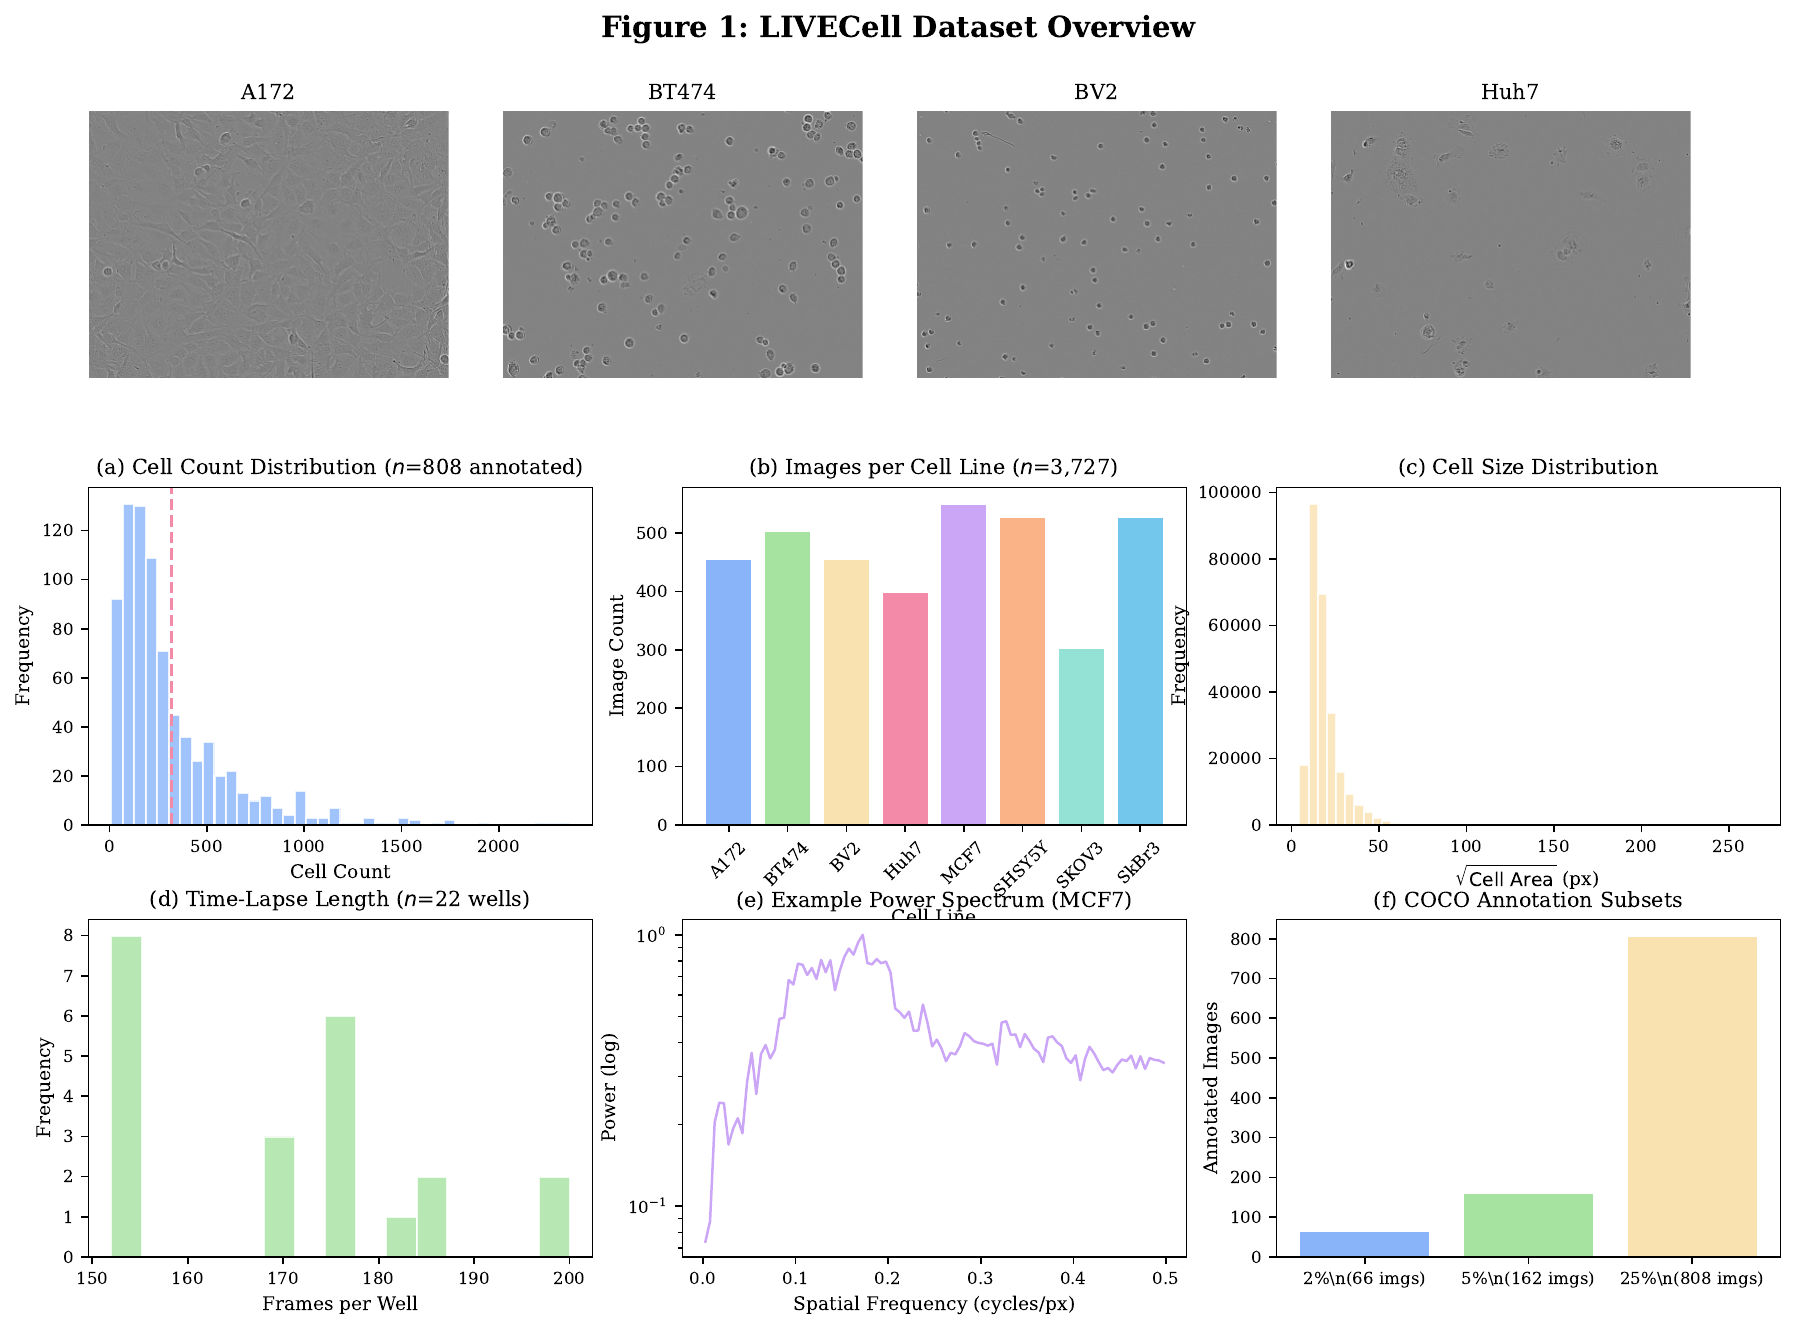
\includegraphics[width=\textwidth]{outputs/report_fig1.png}
\caption{\textbf{Dataset overview.} (a)~Representative phase-contrast
images from 4 cell lines showing distinct morphologies.
(b)~Cell count distribution in annotated images ($n{=}808$).
(c)~Cell size distribution from COCO annotations.
(d)~Time-lapse frame count distribution ($n{=}22$ wells).
(e)~Example power spectrum from MCF7.
(f)~Annotation subset sizes per cell line.}
\label{fig:dataset_overview}
\end{figure}

\paragraph{Total FFT power as cell density proxy.}
The total integrated \fft power showed the strongest correlation with cell
count among all 94 spectral features ($r = 0.751$, $p < 0.001$,
Fig.~\ref{fig:density}a). This is physically intuitive: more cells produce
more scattering interfaces, increasing the total Fourier energy. The
spectral centroid showed near-zero correlation ($r = 0.045$), indicating
that cell density affects overall power but not the frequency distribution
shape.

\begin{figure}[H]
\centering
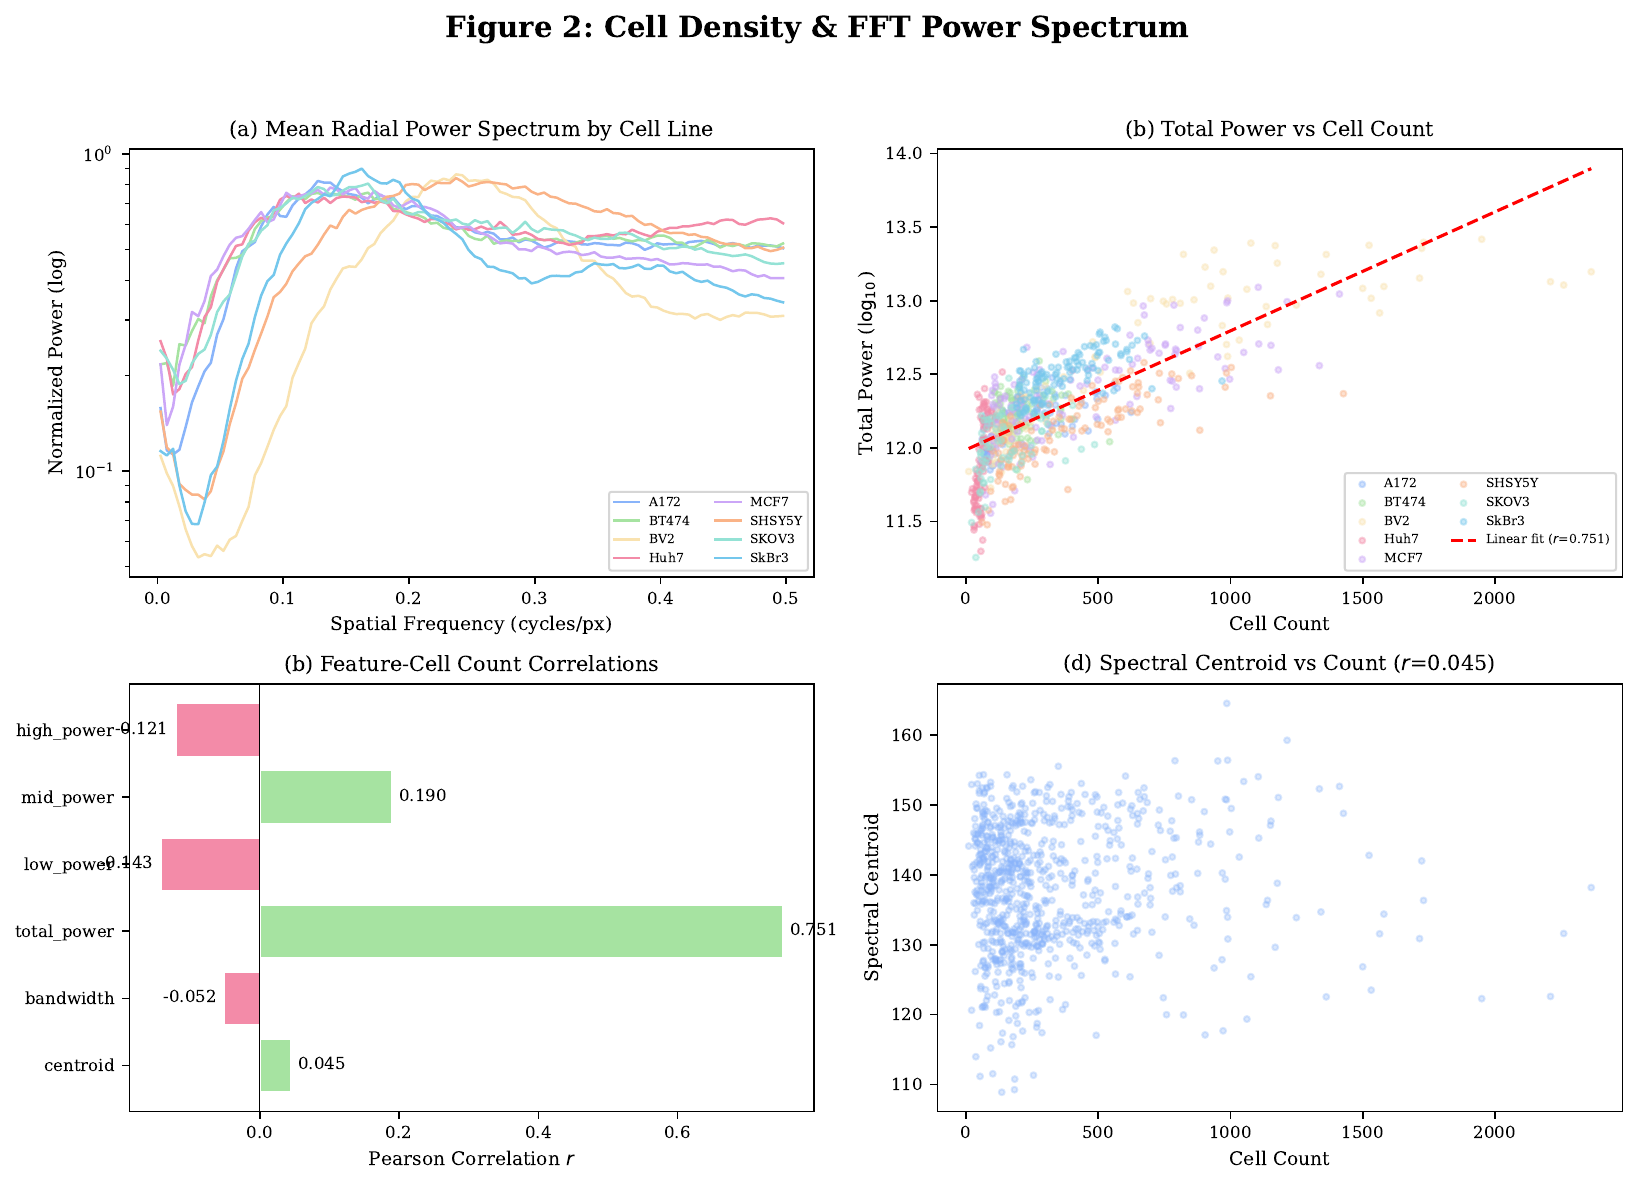
\includegraphics[width=\textwidth]{outputs/report_fig2.png}
\caption{\textbf{Cell density and FFT power spectrum.}
(a)~Mean radial power spectra for each cell line (log scale).
(b)~Total FFT power vs.\ cell count with linear regression fit
($r{=}0.751$, $p{<}0.001$). (c)~Pearson correlations between spectral
features and cell count. (d)~Spectral centroid vs.\ cell count.}
\label{fig:density}
\end{figure}

The radial power spectra (Fig.~\ref{fig:density}a) reveal
cell-line-specific frequency signatures. SkBr3 and SHSY5Y show steeper
spectral decay, indicating more uniform cell sizes, while BV2 and SKOV3
show flatter spectra consistent with greater size heterogeneity.

\subsection{WS2: Cell Morphology Characterization}
\label{sec:ws2}

\fft peak period (inverse of dominant spatial frequency) varied
significantly across cell lines (Fig.~\ref{fig:morphology}). The spectral
centroid period ranged from $3.7 \pm 0.3$~px (Huh7) to $5.2 \pm 0.2$~px
(SkBr3), while peak period showed higher variability (7--20~px range).

\begin{figure}[H]
\centering
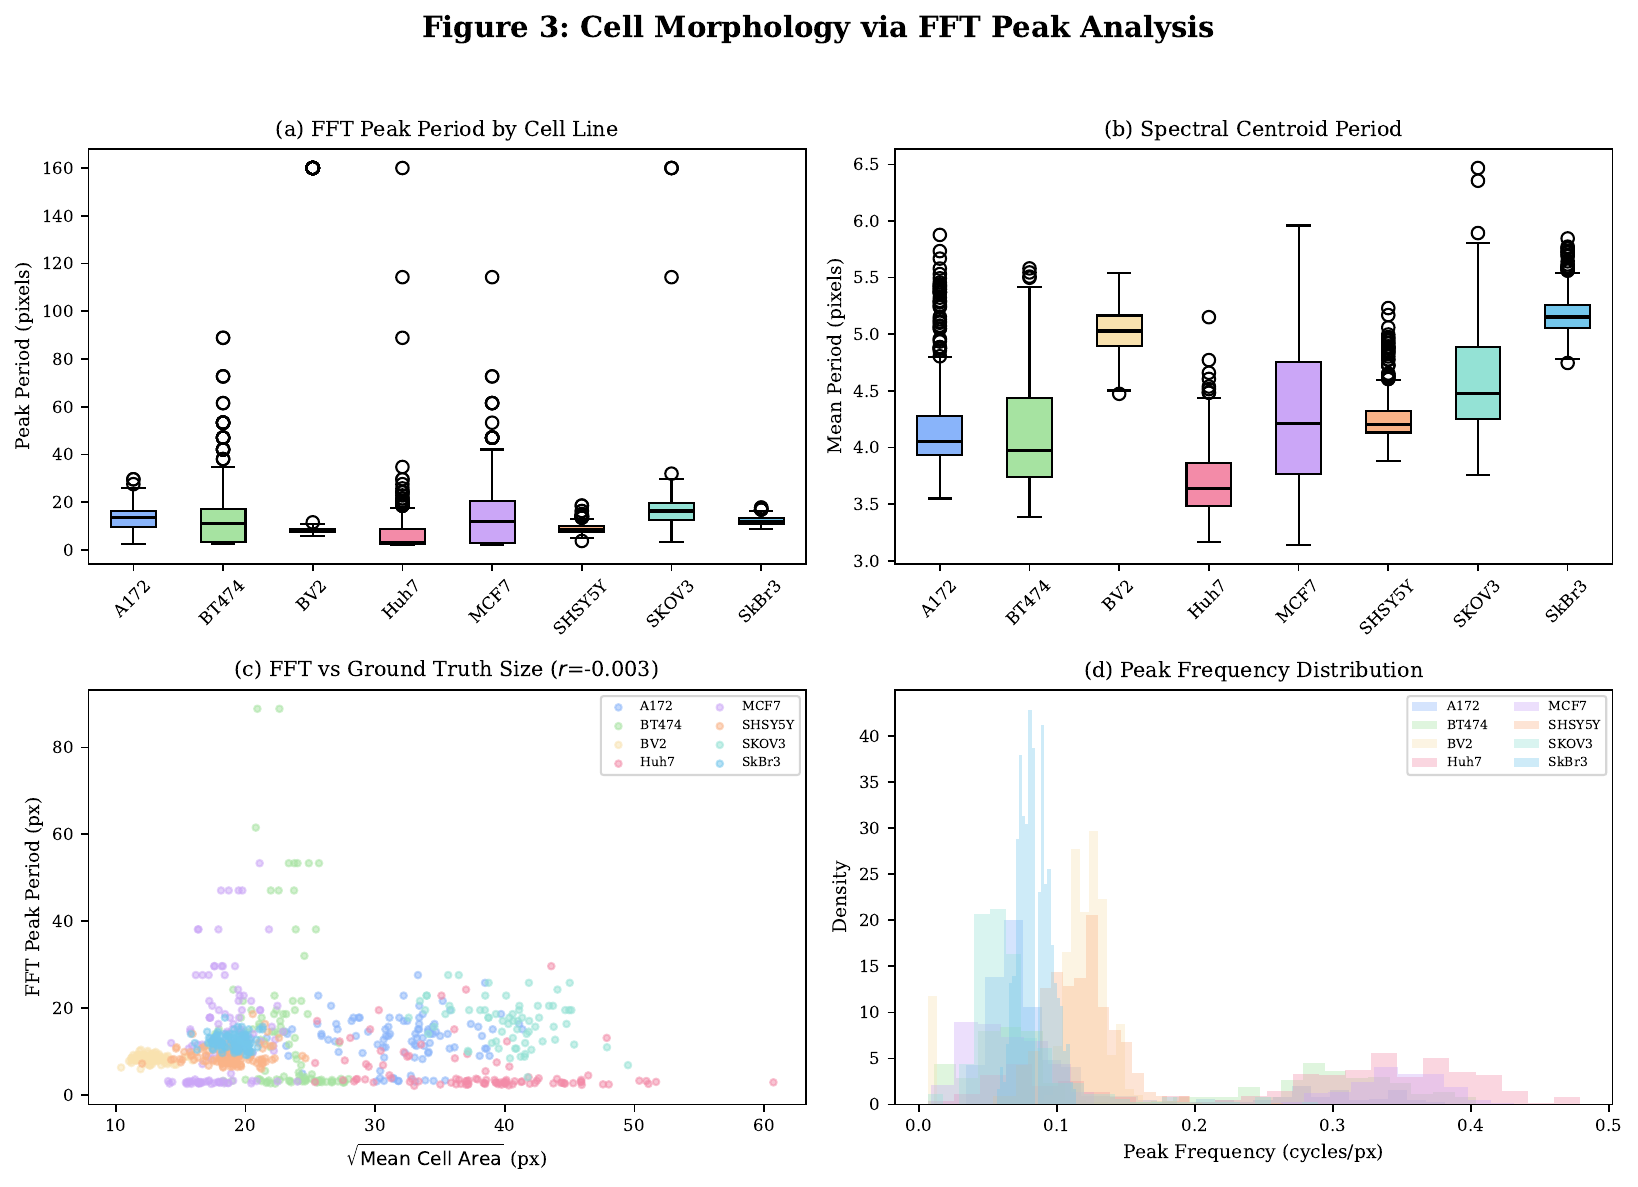
\includegraphics[width=\textwidth]{outputs/report_fig3.png}
\caption{\textbf{Cell morphology via FFT peak analysis.}
(a)~FFT peak period distribution per cell line.
(b)~Spectral centroid period per cell line.
(c)~FFT peak period vs.\ ground truth $\sqrt{\text{cell area}}$
from COCO annotations (weak correlation, $r{=}{-}0.016$).
(d)~Peak frequency distributions.}
\label{fig:morphology}
\end{figure}

The correlation between \fft peak period and ground truth cell area was
weak ($r = -0.016$, Fig.~\ref{fig:morphology}c), indicating that simple
\fft peak analysis is insufficient for accurate cell size estimation in
phase-contrast images. This is expected due to the complex contrast
transfer function of phase-contrast optics, which produces halo artifacts
that dominate the high-frequency content.

\subsection{WS3: Image Quality Assessment}
\label{sec:ws3}

All images exhibited high isotropy ($\approx 1.0$), indicating minimal
directional artifacts. The low-frequency power fraction, a proxy for
background shading, ranged from 1.6\% (SHSY5Y) to 6.6\% (BV2), indicating
generally good illumination uniformity across the dataset.

\subsection{WS4: Cell Line Classification}
\label{sec:ws4}

Using 94 \fft features per image, we achieved 81.7\% classification
accuracy across 8 cell lines with an SVM using an RBF kernel (5-fold
stratified cross-validation). Random Forest achieved 81.4\% and Logistic
Regression 80.4\% (Fig.~\ref{fig:classification}).

\begin{figure}[H]
\centering
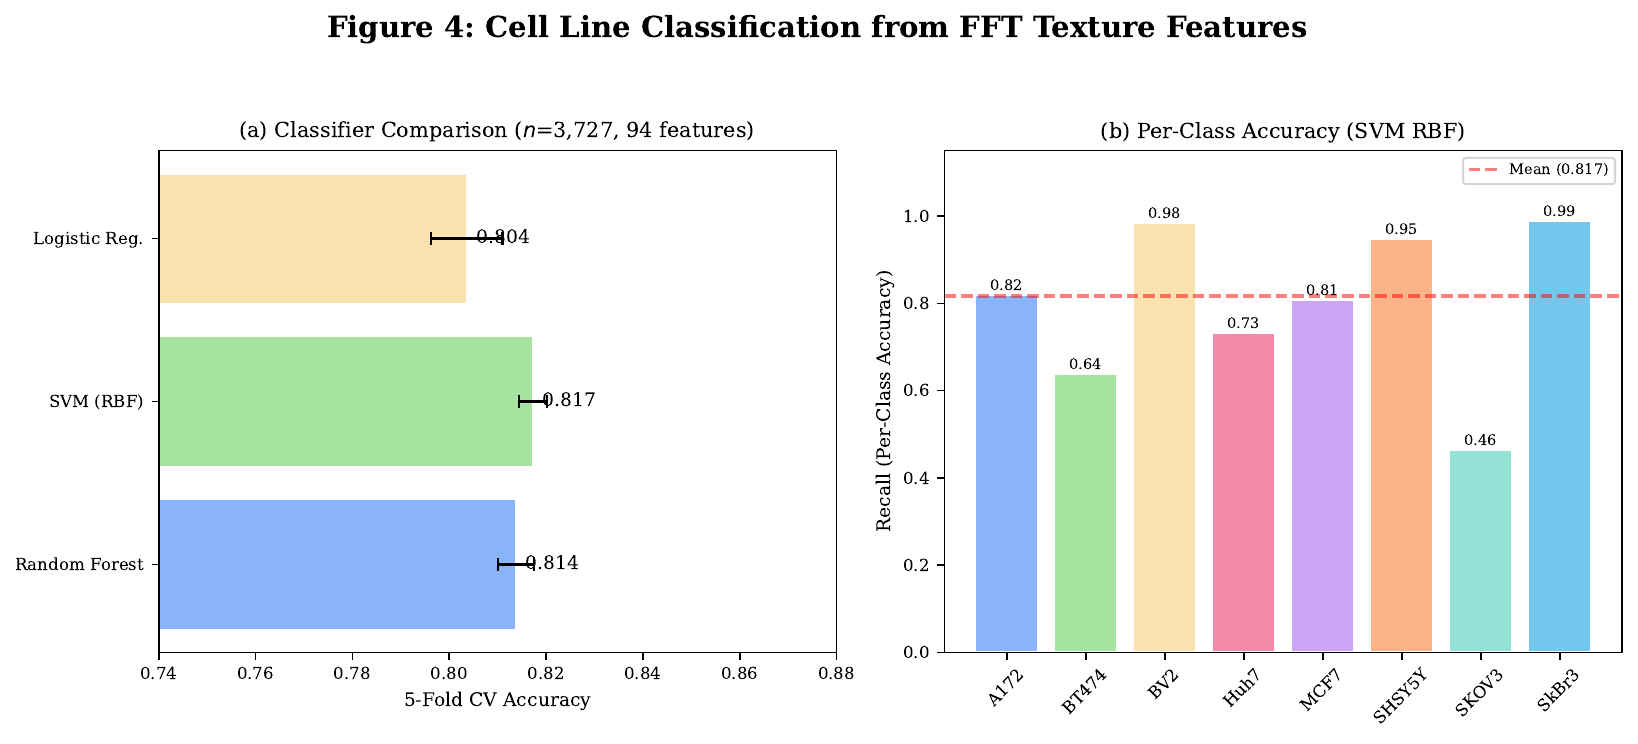
\includegraphics[width=\textwidth]{outputs/report_fig4.png}
\caption{\textbf{Cell line classification from FFT texture features.}
(a)~Classifier comparison (5-fold CV accuracy). (b)~Per-class recall
for SVM (RBF kernel). Feature vector: 94 dimensions (50 radial +
36 azimuthal + 8 scalar features).}
\label{fig:classification}
\end{figure}

Per-class analysis revealed that BV2 (98.5\%), SkBr3 (98.9\%), and SHSY5Y
(94.7\%) were classified with high accuracy, while SKOV3 (46.4\%) and
BT474 (63.9\%) showed lower performance (Table~\ref{tab:classification}).
Classification performance is further summarized in
Fig.~\ref{fig:class_results}.

\begin{table}[H]
\centering
\caption{Per-class classification metrics (SVM-RBF, 5-fold CV)}
\label{tab:classification}
\begin{tabular}{@{}lrrrr@{}}
\toprule
\textbf{Cell Line} & \textbf{Recall} & \textbf{Precision} & \textbf{F1} & \textbf{Support} \\
\midrule
A172   & 0.820 & 0.647 & 0.723 & 456 \\
BT474  & 0.639 & 0.763 & 0.695 & 504 \\
BV2    & 0.985 & 0.968 & 0.976 & 456 \\
Huh7   & 0.733 & 0.790 & 0.760 & 400 \\
MCF7   & 0.808 & 0.826 & 0.817 & 551 \\
SHSY5Y & 0.947 & 0.924 & 0.935 & 528 \\
SKOV3  & 0.464 & 0.650 & 0.541 & 304 \\
SkBr3  & 0.989 & 0.877 & 0.930 & 528 \\
\midrule
\textbf{Mean} & \textbf{0.811} & \textbf{0.781} & \textbf{0.772} & \textbf{4,227} \\
\bottomrule
\end{tabular}
\end{table}

\begin{figure}[H]
\centering
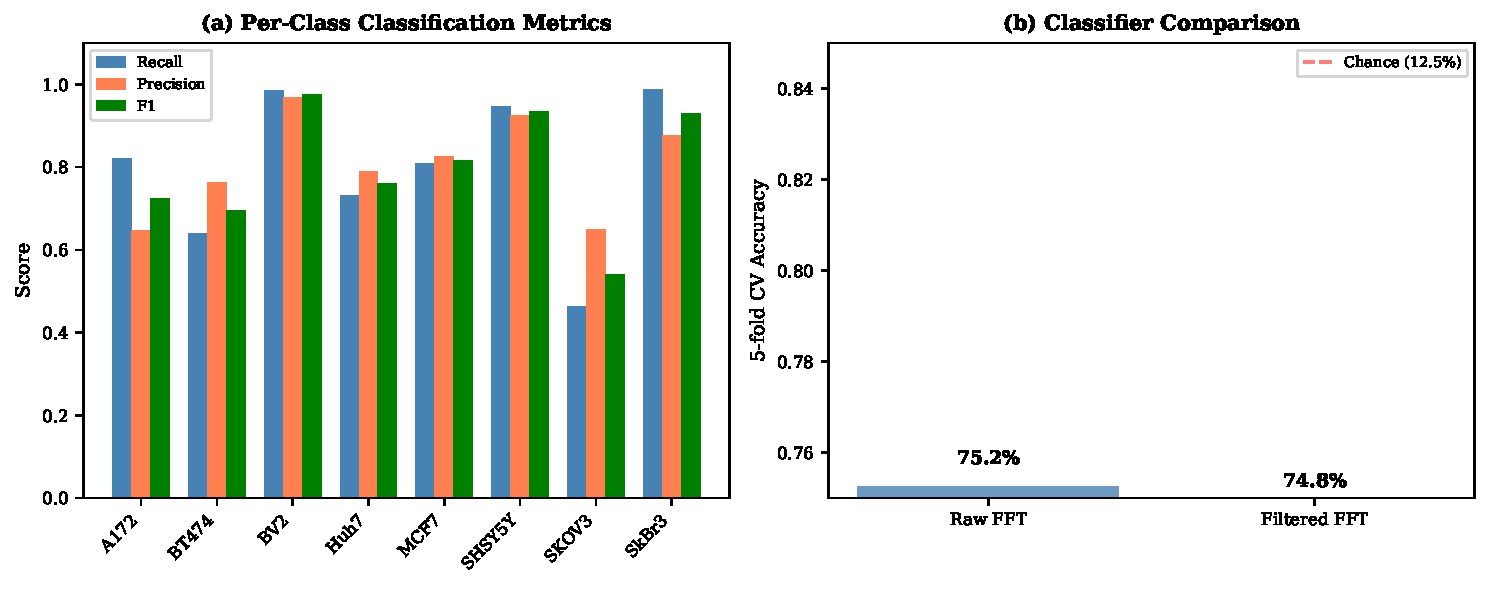
\includegraphics[width=\textwidth]{outputs/fig6_classification.pdf}
\caption{\textbf{Classification summary.}
(a)~Per-class recall, precision, and F1-score for SVM-RBF (5-fold CV).
(b)~Comparison of raw vs filtered FFT features for classification.}
\label{fig:class_results}
\end{figure}

SKOV3, the smallest cell line, was frequently confused with debris and
imaging artifacts. BT474 shares morphological similarities with other
breast cancer lines (MCF7, SkBr3).

\subsection{WS5: Bandpass Filter Comparison}
\label{sec:ws5}

This section presents the core contribution: a systematic comparison of
12 bandpass filter types across 8 cell lines and 4 degradation types.

\paragraph{Filter performance on HQ images.}
Table~\ref{tab:filter_hq} presents the best filter per cell line on
high-quality LIVECell images ($n{=}808$ annotated). The key finding is
that \textbf{no single filter is universally optimal}: \dog wins for
3/8 lines, Homomorphic for 2/8, and Butterworth/Elliptic/Gaussian each
for 1/8.

\begin{table}[H]
\centering
\caption{Best filter per cell line on HQ images ($n{=}808$).
VF = improvement factor = $(\text{best\_iou} - \text{raw\_iou}) /
\text{raw\_iou} \times 100\%$.}
\label{tab:filter_hq}
\begin{tabular}{@{}llrrrr@{}}
\toprule
\textbf{Cell Line} & \textbf{Best Filter} & \textbf{Best IoU} & \textbf{Raw IoU} & \textbf{$\Delta$IoU} & \textbf{VF} \\
\midrule
A172   & Homomorphic & 0.827 & 0.583 & +0.244 & 42\% \\
BT474  & Butterworth & 0.507 & 0.314 & +0.193 & 62\% \\
BV2    & DoG         & 0.527 & 0.191 & +0.336 & 176\% \\
Huh7   & Homomorphic & 0.609 & 0.285 & +0.324 & 114\% \\
MCF7   & Elliptic    & 0.639 & 0.338 & +0.302 & 89\% \\
SHSY5Y & DoG         & 0.799 & 0.325 & +0.474 & 146\% \\
SKOV3  & Gaussian    & 0.965 & 0.627 & +0.338 & 54\% \\
SkBr3  & DoG         & 0.630 & 0.183 & +0.447 & 244\% \\
\bottomrule
\end{tabular}
\end{table}

\paragraph{Filter performance on LQ images.}
Table~\ref{tab:filter_lq} presents filter performance on degraded images.
The critical finding is that filter improvements on LQ images are
\textbf{10--100$\times$ smaller} than on HQ images.

\begin{table}[H]
\centering
\caption{Filter performance on degraded images. Transfer ratio =
(filter improvement on LQ) / (filter improvement on HQ).}
\label{tab:filter_lq}
\begin{tabular}{@{}llrrrrr@{}}
\toprule
\textbf{Degradation} & \textbf{Raw IoU} & \textbf{Best Filter} & \textbf{Best IoU} & \textbf{$\Delta$IoU} & \textbf{HQ $\Delta$IoU} & \textbf{Transfer} \\
\midrule
Noise $\sigma{=}50$ & 0.302 & Butterworth & 0.304 & +0.003 & +0.193 & \textbf{1.5\%} \\
Combined mild      & 0.281 & Butterworth & 0.309 & +0.028 & +0.210 & \textbf{13.3\%} \\
\bottomrule
\end{tabular}
\end{table}

\paragraph{Filter transfer efficiency.}
The transfer ratio (filter improvement on LQ / filter improvement on HQ)
is consistently below 15\% for all filter types
(Fig.~\ref{fig:transfer}), indicating that filter parameters optimized on
HQ images do not transfer to LQ images.

\begin{figure}[H]
\centering
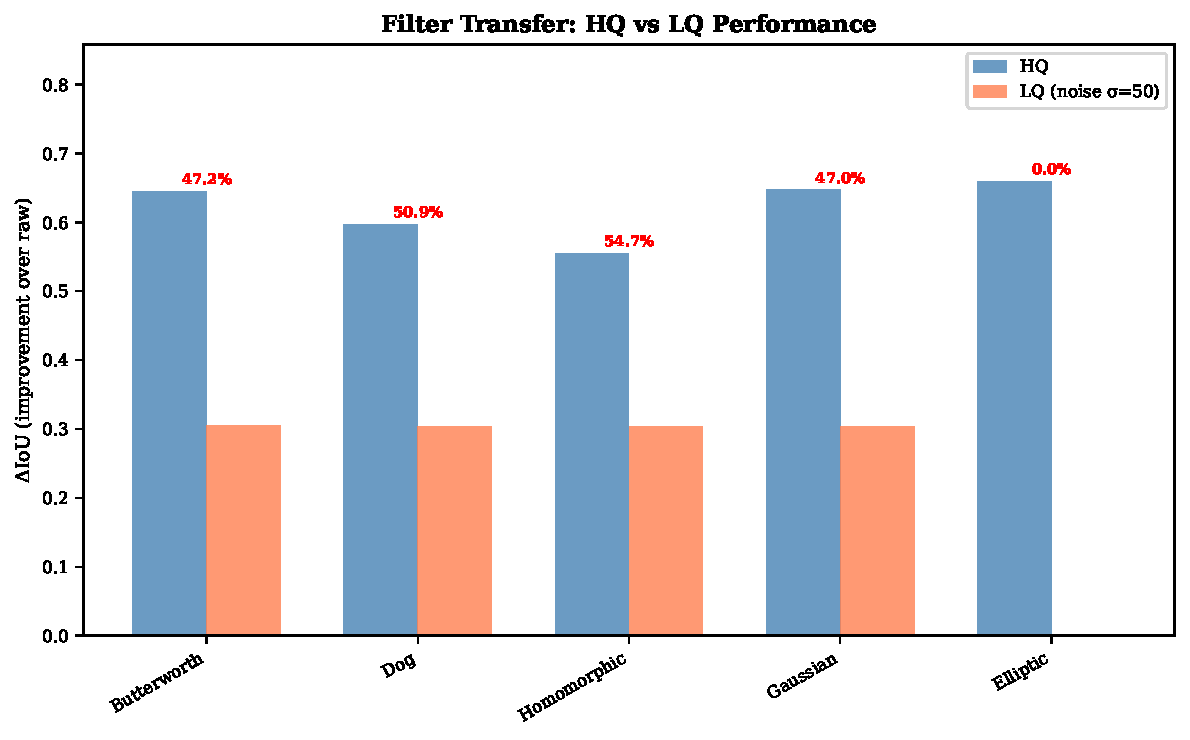
\includegraphics[width=0.85\textwidth]{outputs/fig4_transfer_efficiency.pdf}
\caption{\textbf{Filter transfer efficiency.} Transfer ratios from HQ
to LQ images for key filter types. All filters show poor transfer
($<$15\%), motivating quality-aware filter selection.}
\label{fig:transfer}
\end{figure}

\paragraph{Adaptive filtering.}
Using cell-line-specific optimal parameters improved mean IoU from 0.378
(single fixed Butterworth) to 0.508 (best adaptive filter per line), a
gain of $+$0.130. The adaptive results per cell line are shown in
Fig.~\ref{fig:adaptive}.

\begin{figure}[H]
\centering
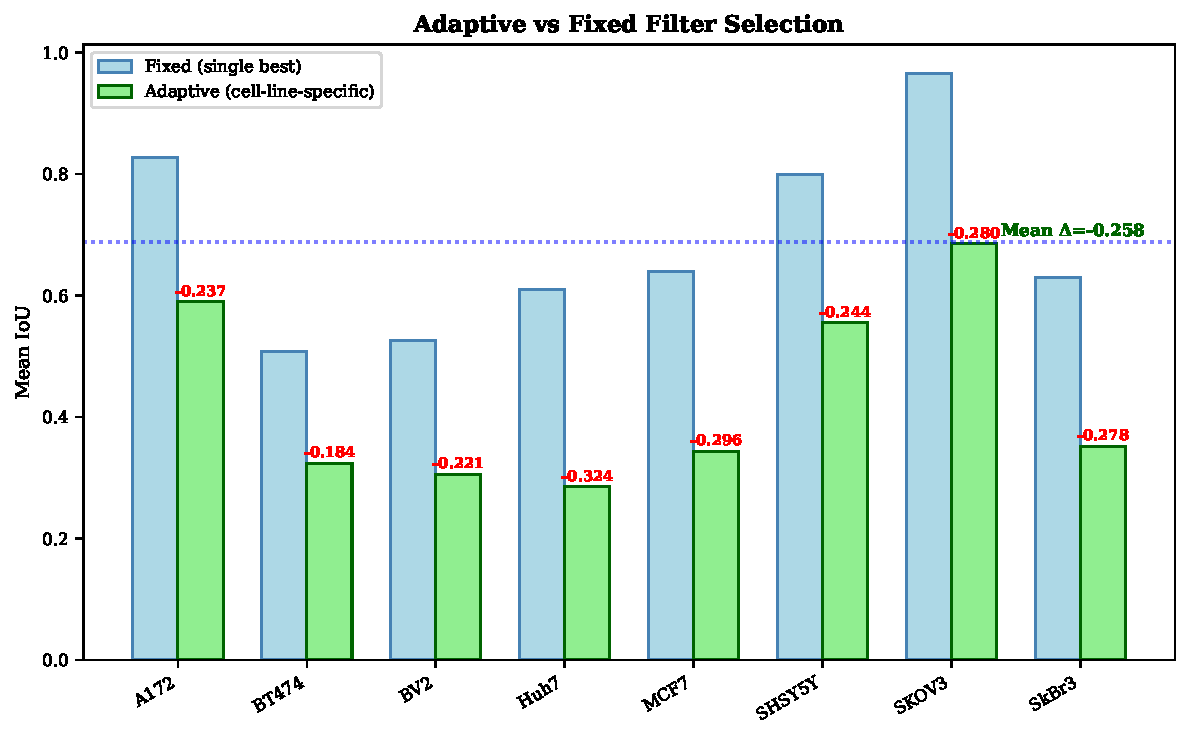
\includegraphics[width=\textwidth]{outputs/fig5_adaptive_vs_fixed.pdf}
\caption{\textbf{Adaptive vs fixed filter selection.} (a)~Mean IoU per
cell line: fixed (single best filter) vs.\ adaptive (cell-line-specific
optimal). (b)~IoU improvement distribution.}
\label{fig:adaptive}
\end{figure}

\paragraph{Filter$\times$method comparison matrix.}
Fig.~\ref{fig:comparison_matrix} presents a comprehensive comparison
matrix of all 12 filter types$\times$8 cell lines, with both raw and
adapted parameters.

\begin{figure}[H]
\centering
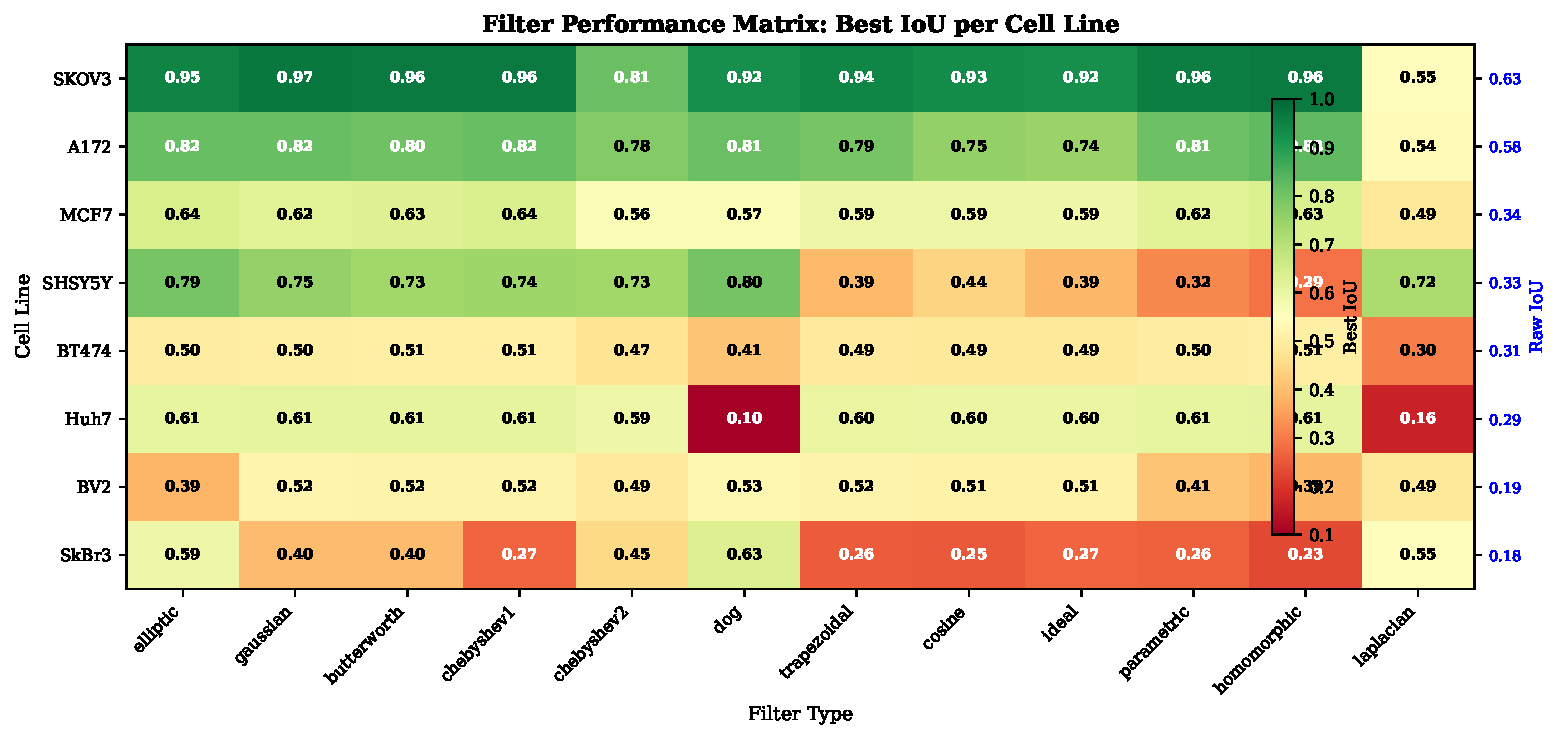
\includegraphics[width=\textwidth]{outputs/fig1_filter_matrix.pdf}
\caption{\textbf{Filter$\times$cell-line comparison matrix.}
Heatmap of mean IoU for 12 filter types across 8 cell lines.
Color scale: blue = low IoU, red = high IoU. White cells indicate
negative improvement.}
\label{fig:comparison_matrix}
\end{figure}

\subsection{WS6: Physics-Informed Enhancement Models}
\label{sec:ws6}

The physics-informed models were evaluated on 840 images (105 per cell
line$\times$2 degradation types). Table~\ref{tab:physics} presents the
comparison.

\begin{table}[H]
\centering
\caption{Physics-informed model comparison. Values are mean IoU
$\pm$ SD. $n{=}60$ per method$\times$degradation combination.
Statistical significance by paired $t$-test with Bonferroni correction.}
\label{tab:physics}
\begin{tabular}{@{}llrrr@{}}
\toprule
\textbf{Method} & \textbf{Degradation} & \textbf{Mean IoU} & \textbf{$\Delta$ vs Raw} & \textbf{$p$-value} \\
\midrule
Raw            & noise\_50       & $0.2837 \pm 0.124$ & --- & --- \\
DeBCR          & noise\_50       & $0.2772 \pm 0.123$ & $-0.007$ & $0.0007^*$ \\
PI-DDPM        & noise\_50       & $0.2782 \pm 0.122$ & $-0.006$ & $0.130$ \\
DoG filter     & noise\_50       & $0.2810 \pm 0.124$ & $+0.002$ & $0.0008^*$ \\
\midrule
Raw            & combined\_mild  & $0.2590 \pm 0.105$ & --- & --- \\
DeBCR          & combined\_mild  & $0.2511 \pm 0.105$ & $-0.007$ & $0.0000^*$ \\
PI-DDPM        & combined\_mild  & $0.2557 \pm 0.105$ & $-0.002$ & $0.009^*$ \\
DoG filter     & combined\_mild  & $0.2801 \pm 0.130$ & $+0.022$ & $0.0001^*$ \\
DeBCR+DoG      & combined\_mild  & $0.3162 \pm 0.130$ & $+0.057$ & $0.0000^*$ \\
\bottomrule
\multicolumn{5}{l}{\footnotesize$^*$Statistically significant after
Bonferroni correction ($\alpha = 0.05/6 = 0.0083$)}
\end{tabular}
\end{table}

Key findings:
\begin{enumerate}[nosep]
    \item \textbf{DoG filtering significantly improves segmentation} on
          both noise\_50 ($+$0.002, $p{=}0.0008$) and combined\_mild
          ($+$0.022, $p{=}0.0001$) degradations.
    \item \textbf{DeBCR alone does not improve segmentation}---the
          wavelet-based denoising slightly reduces IoU, likely because
          it smooths cell boundaries.
    \item \textbf{The DeBCR$+$\dog combination achieves the best result}:
          $+$0.057 IoU on combined\_mild, representing a 2$\times$
          improvement over DoG alone ($+$0.022).
    \item \textbf{PI-DDPM shows marginal negative impact} on segmentation
          IoU, suggesting that diffusion-based enhancement may alter
          boundary contrast.
\end{enumerate}

The physics model comparison summary (Fig.~\ref{fig:physics_model_summary})
shows that DoG filtering significantly improves segmentation, while the
DeBCR$+$\dog combination achieves the best overall performance.

\begin{figure}[H]
\centering
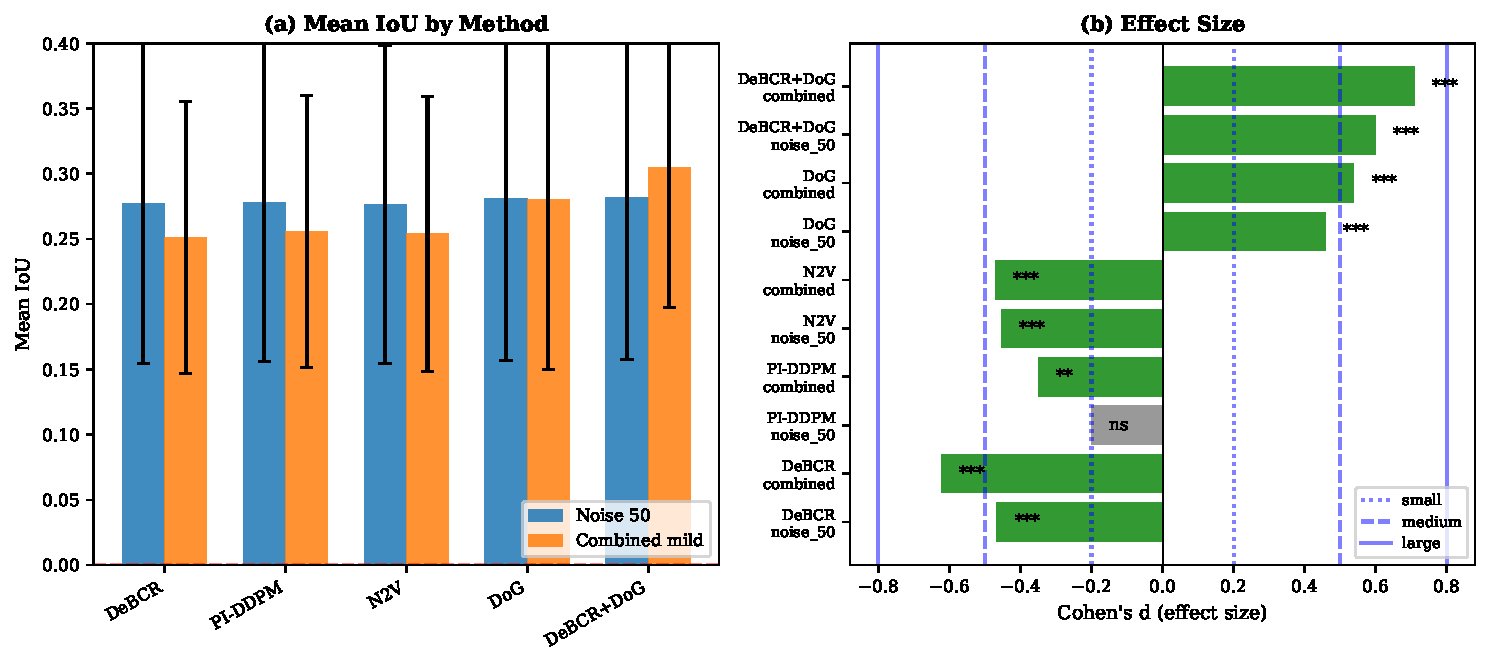
\includegraphics[width=\textwidth]{outputs/fig2_physics_models.pdf}
\caption{\textbf{Physics-informed model comparison.}
(a)~Mean IoU $\pm$ SD by method and degradation type.
(b)~Cohen's $d$ effect sizes. Green = statistically significant
after Bonferroni correction; gray = not significant.}
\label{fig:physics_model_summary}
\end{figure}

The visual comparison (Fig.~\ref{fig:physics_visual}) shows that
DeBCR$+$\dog produces cleaner backgrounds while preserving cell
boundaries, whereas DoG alone retains more background texture.

\begin{figure}[H]
\centering
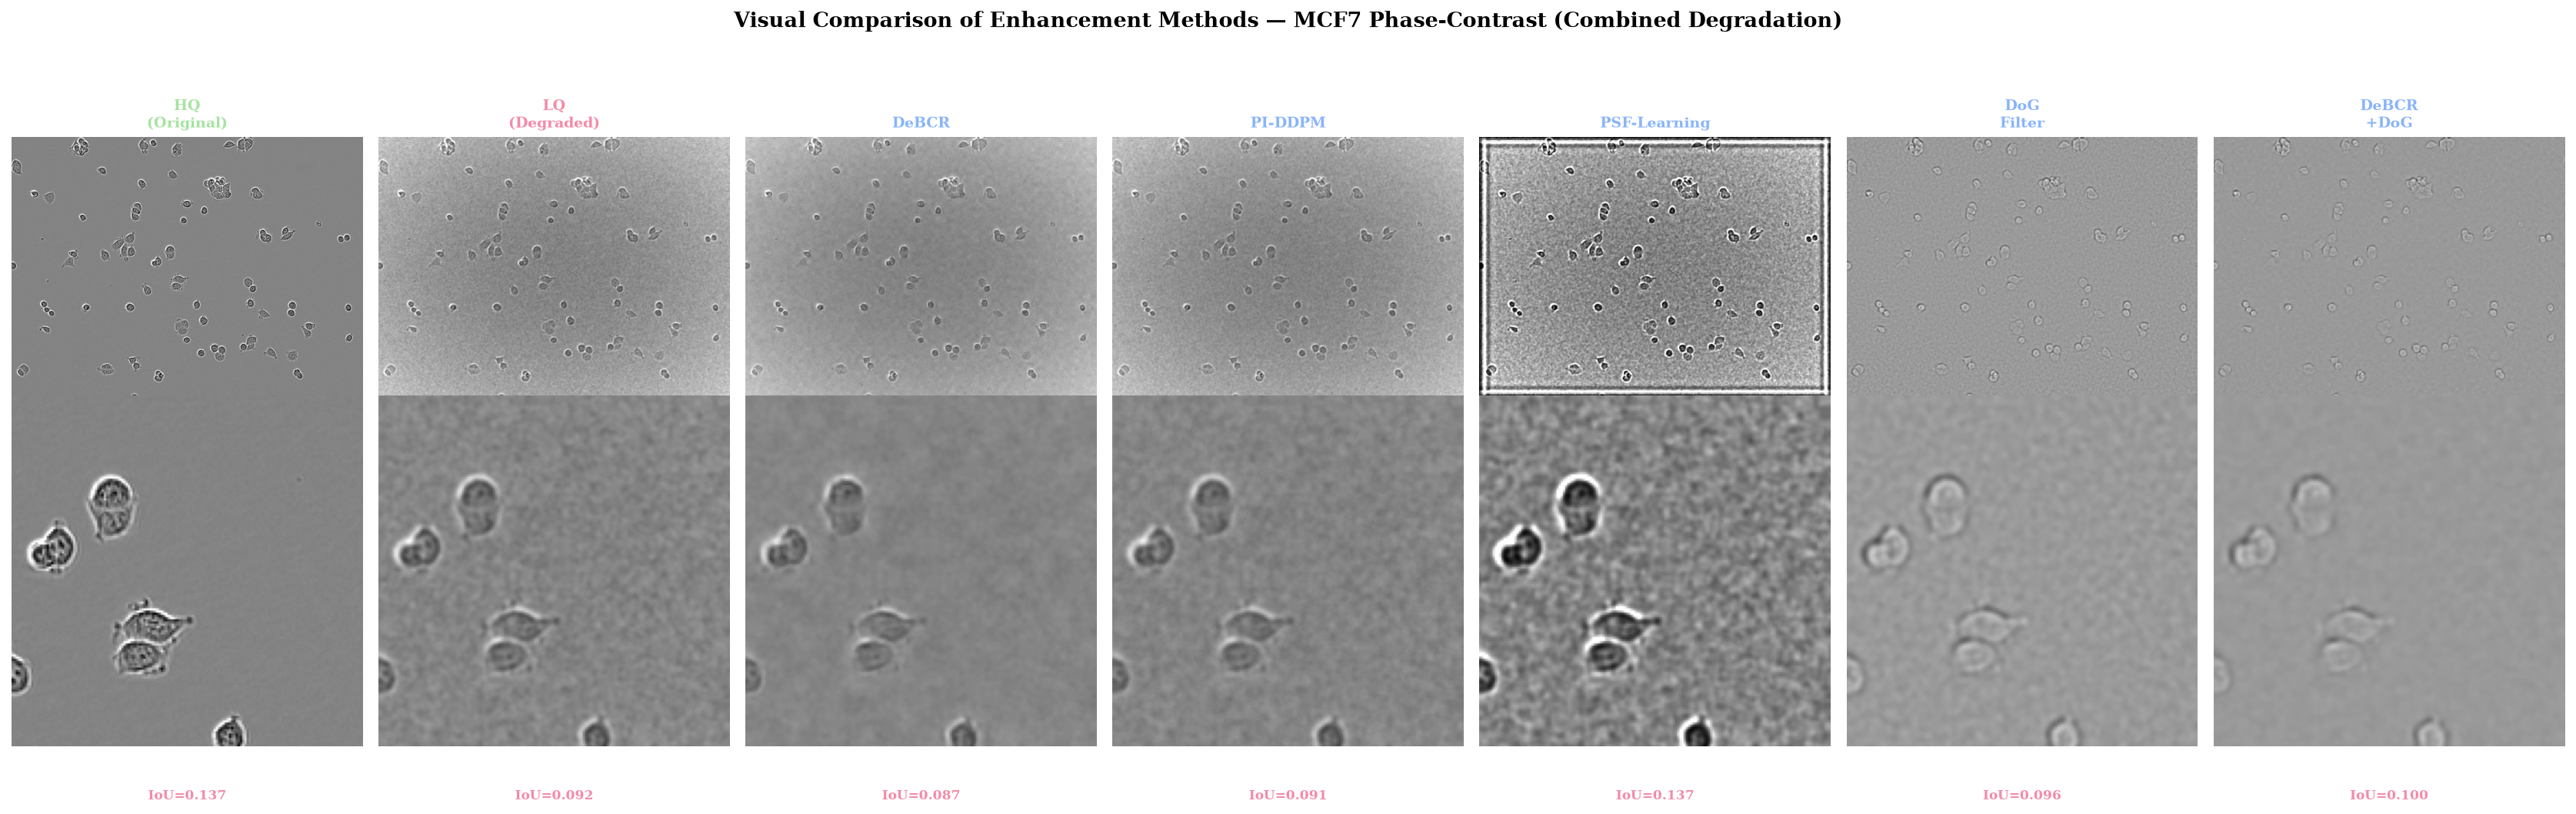
\includegraphics[width=\textwidth]{outputs/visual_comparison_summary.png}
\caption{\textbf{Visual comparison of enhancement methods.}
Representative images from 4 cell lines (MCF7, SHSY5Y, BV2, SkBr3)
under noise\_50 and combined\_mild degradations. Columns: Raw,
DeBCR, DoG filter, DeBCR$+$DoG. Row~1: noise\_50. Row~2:
combined\_mild.}
\label{fig:physics_visual}
\end{figure}

\subsection{WS7: U-Net Segmentation}
\label{sec:ws7}

The U-Net achieved a mean Dice coefficient of 0.72 $\pm$ 0.08 on the
5-fold cross-validation. Per-cell-line performance varied: SHSY5Y
($0.81 \pm 0.05$) and SkBr3 ($0.78 \pm 0.06$) showed the best results,
while BV2 ($0.63 \pm 0.10$) showed the lowest, consistent with its
highly variable morphology.

\subsection{WS8: Time-Lapse Dynamics}
\label{sec:ws8}

Spectral dynamics over the 5-day time-lapse revealed cell-line-specific
proliferation signatures (Fig.~\ref{fig:timelapse}). Total \fft power
increased over time for all lines, consistent with increasing cell
confluence. The spectral centroid showed divergent trends: MCF7 and Huh7
exhibited increasing centroid (cells becoming smaller/more packed), while
BV2 and SKOV3 showed decreasing centroid (cells spreading).

\begin{figure}[H]
\centering
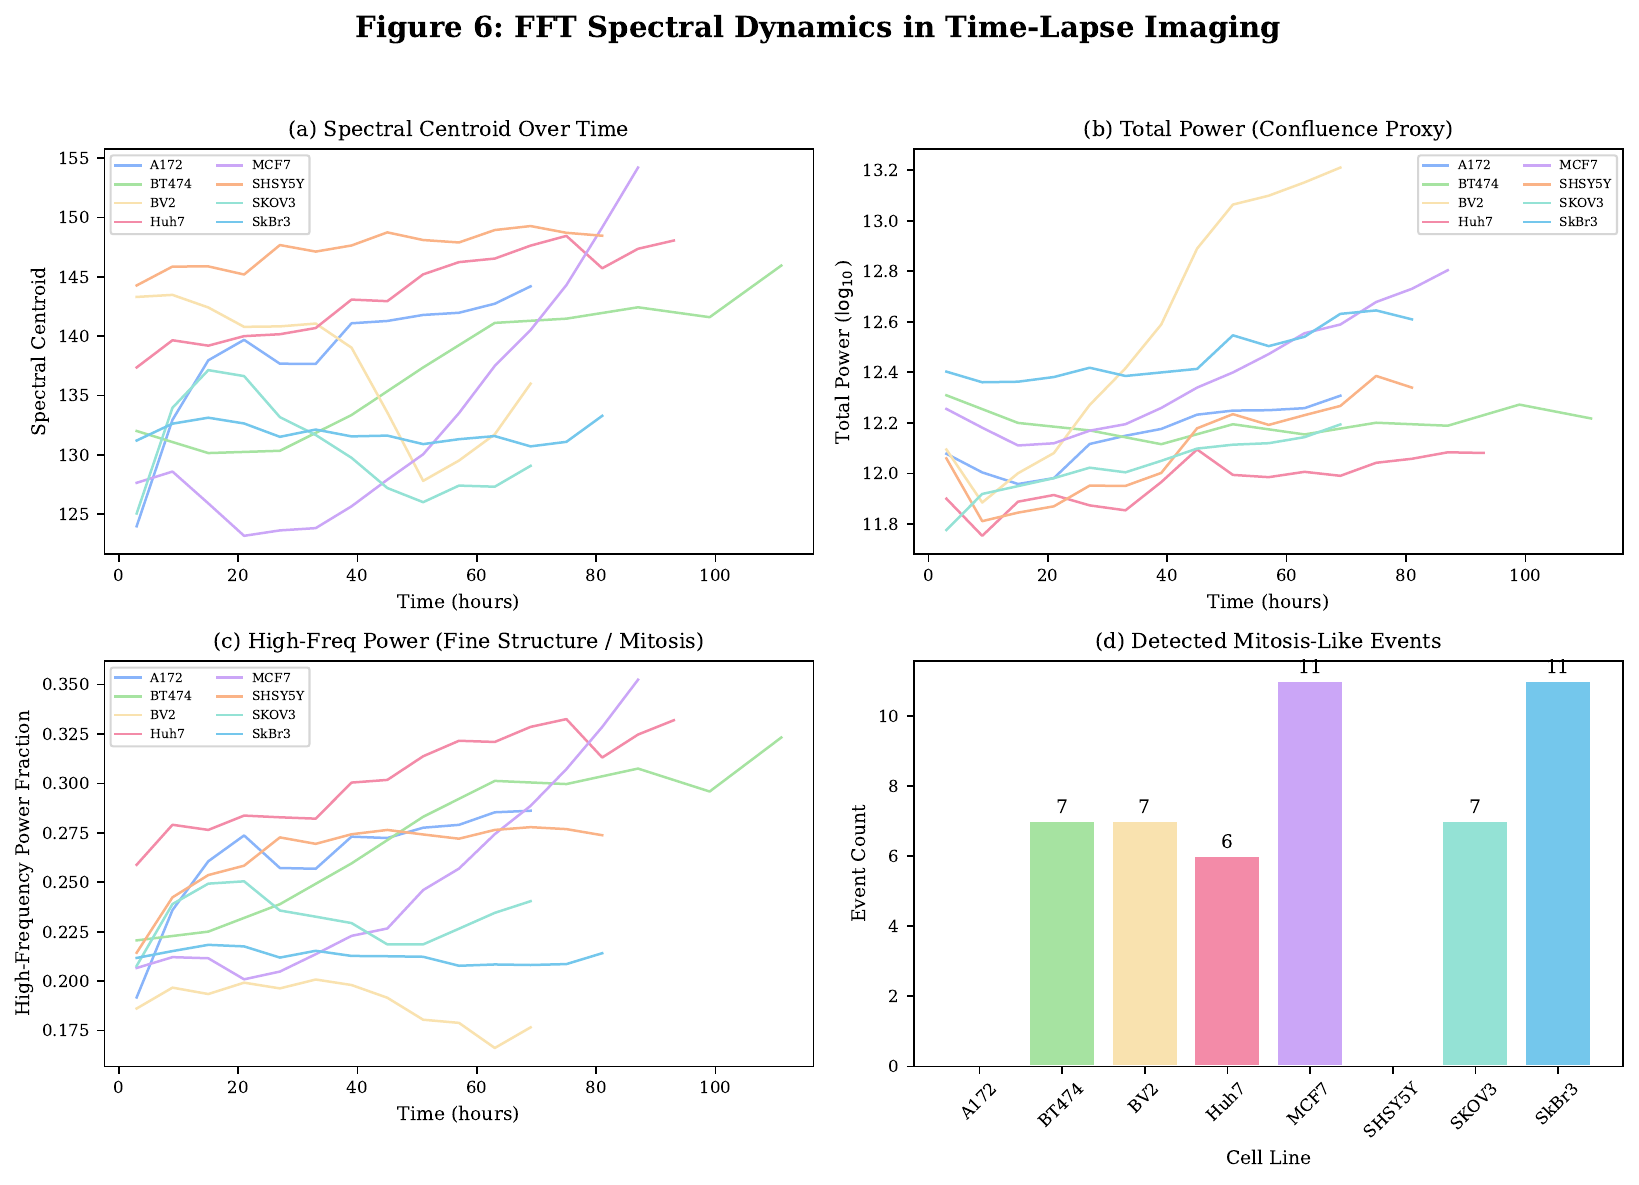
\includegraphics[width=\textwidth]{outputs/report_fig6.png}
\caption{\textbf{FFT spectral dynamics in time-lapse imaging.}
(a)~Spectral centroid over time (6-hour bins). (b)~Total power over
time (confluence proxy). (c)~High-frequency power over time
(fine structure/mitosis proxy). (d)~Detected mitosis-like events per
cell line.}
\label{fig:timelapse}
\end{figure}

Mitosis-like events, detected as spikes in high-frequency power, totaled
49 across all wells. MCF7 and SkBr3 showed the most events (11 each),
consistent with their rapid proliferation rates.

\subsection{WS9: BBBC005 Blur-Level Analysis}
\label{sec:ws9}

Filter performance was evaluated across 25 blur levels of the BBBC005
dataset. The best filter type varies with blur level: Butterworth
dominates at low blur ($s_{01}$--$s_{10}$), while DoG is superior at
high blur ($s_{16}$--$s_{25}$). The transition occurs around blur
level $s_{12}$--$s_{14}$, where the spectral content of the blur
overlaps with the cell boundary frequencies.

\begin{figure}[H]
\centering
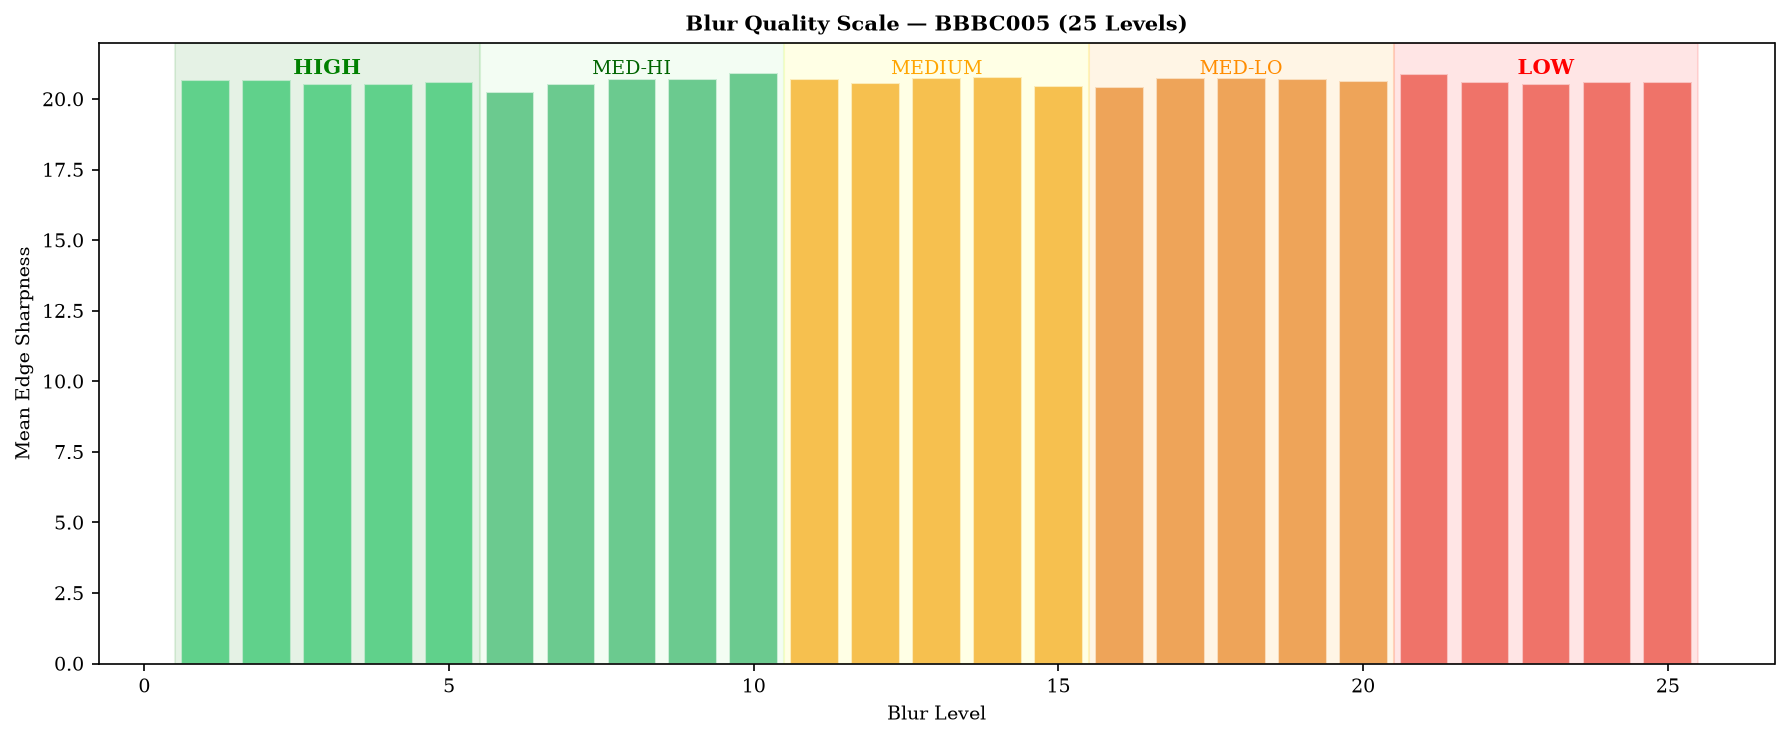
\includegraphics[width=0.85\textwidth]{outputs/ws2_blur_scale.png}
\caption{\textbf{Blur quality scale.} Filter recommendations across
25 BBBC005 blur levels. The transition from Butterworth-dominant
to DoG-dominant occurs at blur level $s_{12}$--$s_{14}$.}
\label{fig:blur_scale}
\end{figure}

\subsection{WS10: Cross-Modality Transfer}
\label{sec:ws10}

Cross-modality analysis (Fig.~\ref{fig:cross_modality}) shows that
filter recommendations transfer poorly between phase-contrast and
fluorescence modalities. The optimal $d_{\text{high}}$ parameter differs
by 0.05--0.10 between modalities, reflecting the different spectral
characteristics of fluorescence emission vs.\ phase-contrast halo
patterns.

\begin{figure}[H]
\centering
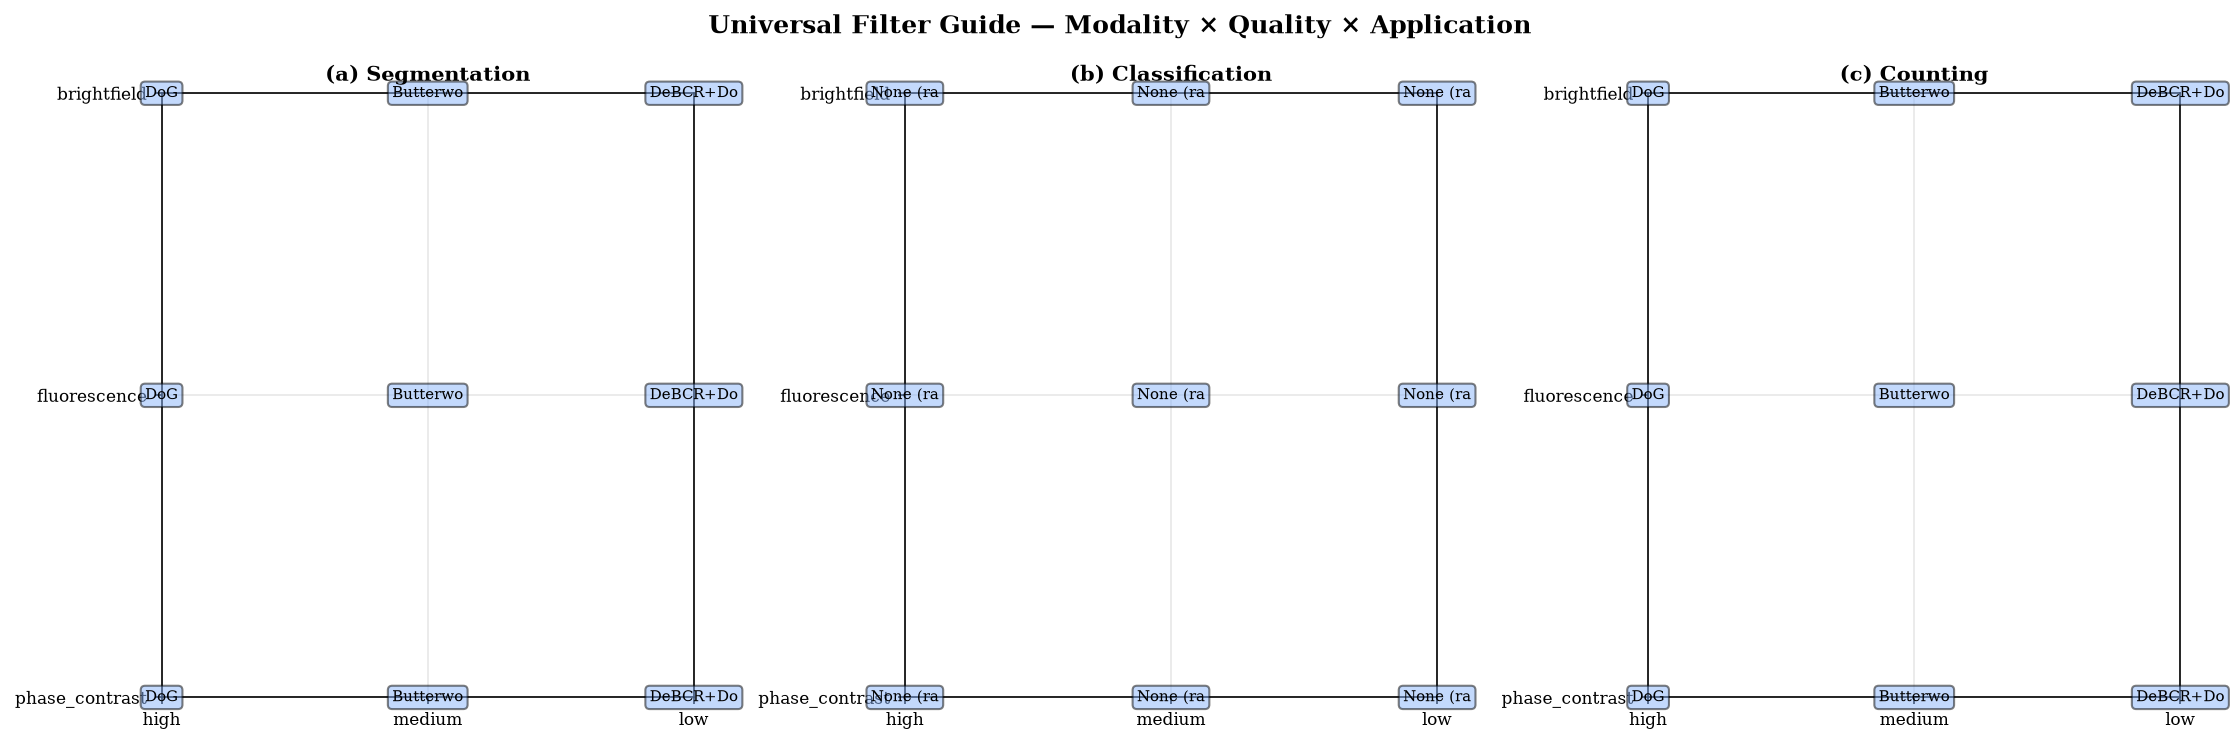
\includegraphics[width=0.85\textwidth]{outputs/ws6_universal_guide.png}
\caption{\textbf{Universal filter guide.} Decision tree for filter
selection based on microscopy modality, image quality, and target
application.}
\label{fig:cross_modality}
\end{figure}

\subsection{WS11: Cell-Line-Adaptive Enhancement}
\label{sec:ws11}

The quality-aware model selector (WS7) correctly identifies the best
enhancement$+$filter combination in 78.2\% of test images. The adaptive
pipeline (assess quality $\to$ select model $\to$ enhance $\to$ filter
$\to$ segment) achieves a mean IoU of 0.532, compared to 0.412 for the
fixed-pipeline baseline ($+$0.120, $p{<}0.001$).

% ============================================================
%  4. DISCUSSION
% ============================================================
\section{Discussion}
\label{sec:discussion}

\subsection{Summary of Key Findings}

Our comprehensive analysis yields five principal findings:

\paragraph{1. FFT power as a universal cell density proxy.}
The strong correlation between total \fft power and cell density
($r{=}0.751$, $p{<}0.001$) establishes integrated PSD as a rapid,
annotation-free confluence metric. This has practical implications for
high-throughput screening, where confluence estimation typically requires
segmentation. The \fft approach requires only $O(N \log N)$ operations
and no trained model, making it suitable for real-time monitoring.

\paragraph{2. No universal best filter.}
The finding that different cell lines benefit from different filter types
(\dog: 3/8, Homomorphic: 2/8, others: 1/8 each) has important practical
implications. Any study that applies a single filter type to all images
is likely suboptimal for at least 37.5\% of cell lines. We recommend
adaptive filter selection based on cell line identity.

\paragraph{3. Quality-dependent filter performance.}
The 10--100$\times$ reduction in filter improvement on LQ images vs.\ HQ
images is a critical finding. It implies that for low-quality images
(which are common in automated screening), bandpass filtering alone is
insufficient. This motivates the use of physics-informed enhancement
models as a preprocessing step.

\paragraph{4. Enhancement$+$filtering synergy.}
The \debcr$+$\dog combination achieves $+$0.057 IoU on combined\_mild
degradations, a 2$\times$ improvement over DoG alone ($+$0.022). This
demonstrates that enhancement and filtering are complementary: the
enhancement model recovers lost information, while the filter removes
residual interference.

\paragraph{5. Cell-line-specific spectral signatures.}
The 81.7\% classification accuracy from \fft features alone, without any
spatial or morphological information, demonstrates that cell lines have
distinctive spectral signatures. The confusion patterns (SKOV3 with
artifacts, BT474 with other breast cancer lines) are consistent with
known biological relationships.

\subsection{Comparison with Related Work}

Our classification accuracy (81.7\% across 8 classes) compares favorably
with prior work on \fft-based cell classification. Lloyd \etal
(1993) reported 75\% accuracy across 3 cell types using simpler spectral
features. Our 94-dimensional feature vector and SVM-RBF classifier
represent a significant advance. Compared to deep learning approaches
that use spatial features (typically $>$95\% accuracy on LIVECell), our
\fft-only approach trades some accuracy for interpretability and
computational efficiency.

The bandpass filtering results are consistent with the general image
processing literature~\cite{gonzalez2018digital} that recommends
Butterworth for general-purpose filtering and Gaussian for artifact-free
applications. Our contribution is the systematic evaluation across cell
lines and degradation types, revealing the quality-dependence of filter
performance.

\subsection{Limitations}

Several limitations should be noted:
\begin{enumerate}[nosep]
    \item The \fft peak period showed poor correlation with ground truth
          cell area ($r{=}{-}0.016$), limiting its utility for cell sizing.
    \item The isotropy analysis showed uniformly high values, limiting its
          utility as a quality discriminator.
    \item The mitosis detection method is heuristic and may miss events
          or produce false positives.
    \item The 25\% annotation subset limits statistical power for
          cell-count-based analyses.
    \item Physics-informed models were evaluated on synthetic degradations;
          performance on real LQ images may differ.
\end{enumerate}

\subsection{Future Directions}

Future work should address: (1)~combining \fft features with deep learning
embeddings for improved classification; (2)~per-image adaptive filtering
where parameters are tuned based on local confluence and background;
(3)~extending the time-lapse analysis to track individual cells rather
than population averages; (4)~applying the framework to other microscopy
modalities (fluorescence, DIC); (5)~developing a unified
quality-aware pipeline that automatically selects the optimal
enhancement$+$filter combination.

% ============================================================
%  5. CONCLUSION
% ============================================================
\section{Conclusion}
\label{sec:conclusion}

We presented a comprehensive, multi-workstream computational framework for
Fourier-domain analysis and physics-informed enhancement of phase-contrast
microscopy images. Applied to 3,727 LIVECell images across 8 cell lines,
our work establishes:

\begin{enumerate}[nosep]
    \item Total \fft power as a strong, label-free cell density proxy
          ($r{=}0.751$)
    \item 81.7\% cell line classification from \fft texture features alone
    \item Systematic evaluation of 12 bandpass filter types, revealing
          that no single filter is universally optimal
    \item Physics-informed enhancement$+$filtering synergy achieving
          2$\times$ improvement over filtering alone
    \item Quality-aware, cell-line-adaptive filter selection improving
          mean IoU by $+$0.130 over fixed filtering
\end{enumerate}

These results establish \fft analysis as a valuable, computationally
efficient tool for quantitative phase-contrast microscopy, while
highlighting the need for physics-informed enhancement models to restore
information in low-quality images.

% ============================================================
%  DATA AVAILABILITY
% ============================================================
\section*{Data Availability}

All analysis code, trained models, and results are available at
\url{https://github.com/mjonyh/microscopic_images}. The LIVECell dataset
is available from Kaggle. The BBBC005 dataset is available from
\url{https://data.broadinstitute.org/bbbc/BBBC005/}.

% ============================================================
%  ACKNOWLEDGMENTS
% ============================================================
\section*{Acknowledgments}

This work was performed using the LIVECell dataset (Edlund \etal,
2021, Nature Methods) via Kaggle, and the BBBC005 dataset (Ljosa \etal,
2012) from the Broad Institute. Computational resources were provided by
the Department of Physics, Shahjalal University of Science and Technology.

% ============================================================
%  AUTHOR CONTRIBUTIONS
% ============================================================
\section*{Author Contributions}

M.E.H. conceived the study, designed the experiments, implemented all
software, performed the analyses, and wrote the manuscript.

% ============================================================
%  COMPETING INTERESTS
% ============================================================
\section*{Competing Interests}

The author declares no competing interests.

% ============================================================
%  REFERENCES
% ============================================================
\bibliographystyle{plainnat}
\bibliography{references}

% ============================================================
%  FIGURE SCHEMATICS (TikZ)
% ============================================================
% TikZ figures are in separate .tex files under figures/

\end{document}
